\documentclass{article}
\usepackage[a4paper,left=3cm, right=3cm, top=2cm, bottom=2cm]{geometry}
\usepackage{amsmath}
\usepackage{graphicx}
\usepackage{caption}
\usepackage{setspace}
\usepackage{xcolor}
\usepackage{titlesec}
\usepackage{amssymb}
\graphicspath{{graph/}}
\title{10.2 Calculus with Parametric Curves}
\date{}
\author{}
\setstretch{1.2} 

% \subsection* 형식 지정 (번호 없음)
\titleformat{name=\section, numberless}
  {\normalfont\large\bfseries\color{blue}}
  {}
  {0pt}
  {}
\geometry{a4paper, margin=1in}

\begin{document}
\maketitle


Having seen how to represent curves by parametric equations, we now apply the methods of calculus to these parametric curves. In particular, we solve problems involving tangents, areas, arc length, speed, and surface area.

\section*{Tangents}
Suppose $f$ and $g$ are differentiable functions and we want to find the tangent line at a point on the parametric curve $x=f(t)$, $y=g(t)$, where $y$ is also a differentiable function of $x$. The Chain Rule gives:
\[
\frac{dy}{dt} = \frac{dy}{dx} \cdot \frac{dx}{dt}
\]
If $\frac{dx}{dt} \neq 0$, we can solve for $\frac{dy}{dx}$:
\[
\frac{dy}{dx} = \frac{dy/dt}{dx/dt}, \quad \text{if } \frac{dx}{dt} \neq 0
\]
This formula enables us to find the slope of the tangent to a parametric curve without having to eliminate the parameter $t$. 
\\The curve has a horizontal tangent when $\frac{dy}{dt} = 0$ (provided $\frac{dx}{dt} \neq 0$), and it has a vertical tangent when $\frac{dx}{dt} = 0$ (provided $\frac{dy}{dt} \neq 0$).

The second derivative can be found by replacing $y$ by $\frac{dy}{dx}$ in the formula:
\[
\frac{d^2y}{dx^2} = {\dfrac{\dfrac{d}{dt}\left(\dfrac{dy}{dx}\right)}{\dfrac{dx}{dt}}}
\]

\subsubsection*{EXAMPLE 1}
A curve C is defined by the parametric equations $x=t^2, y=t^3-3t$.
\begin{enumerate}
    \item[(a)] Show that C has two tangents at the point (3,0) and find their equations.
    \item[(b)] Find the points on C where the tangent is horizontal or vertical.
    \item[(c)] Determine where the curve is concave upward or downward.
    \item[(d)] Sketch the curve.
\end{enumerate}

\paragraph{Solution:}
(a) The point (3,0) corresponds to parameter values $t=\sqrt{3}$ and $t=-\sqrt{3}$. The derivative is:
\[
\frac{dy}{dx} = \frac{dy/dt}{dx/dt} = \frac{3t^2-3}{2t}
\]
For $t=\sqrt{3}$, the slope is $\frac{dy}{dx} = 2\sqrt{3}$. For $t=-\sqrt{3}$, the slope is $\frac{dy}{dx} = -2\sqrt{3}$.
The tangent lines are $y = 2\sqrt{3}(x-3)$ and $y = -2\sqrt{3}(x-3)$.

(b) The tangent is horizontal when $\frac{dy}{dt} = 3t^2-3 = 0$, so $t=\pm 1$. The points are $(1,-2)$ and $(1,2)$. The tangent is vertical when $\frac{dx}{dt} = 2t = 0$, so $t=0$. The point is $(0,0)$.

(c) The second derivative is:
\[
\frac{d^2y}{dx^2} = \dfrac{\dfrac{d}{dt}\left(\dfrac{3t^2-3}{2t}\right)}{2t} = \frac{\dfrac{6t(2t) - 2(3t^2-3)}{(2t)^2}}{2t} = \frac{6t^2+6}{8t^3} = \frac{3(t^2+1)}{4t^3}
\]
The curve is concave upward when $\frac{d^2y}{dx^2} > 0$, which means $t > 0$. It is concave downward when $t < 0$.

(d) The curve is sketched below, showing the points and tangents found in parts (a) and (b).
\begin{figure}[htbp]
    \centering
    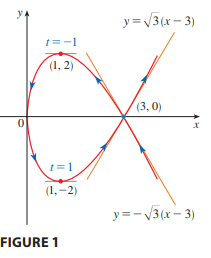
\includegraphics[width=0.3\textwidth]{graph27.png}
\end{figure}

\subsubsection*{EXAMPLE 2}
\begin{enumerate}
    \item[(a)] Find the tangent to the cycloid $x=r(\theta-\sin\theta)$, $y=r(1-\cos\theta)$ at $\theta=\pi/3$.
    \item[(b)] At what points is the tangent horizontal? When is it vertical?
\end{enumerate}
\paragraph{Solution:}
(a) The slope is $\dfrac{dy}{dx} = \dfrac{dy/d\theta}{dx/d\theta} = \dfrac{r\sin\theta}{r(1-\cos\theta)} = \dfrac{\sin\theta}{1-\cos\theta}$. At $\theta=\pi/3$, the slope is $\dfrac{\sqrt{3}/2}{1-1/2} = \sqrt{3}$. The point is $(r(\pi/3 - \sqrt{3}/2), r/2)$. The tangent equation is $y - \frac{r}{2} = \sqrt{3}\left(x - r\left(\frac{\pi}{3} - \frac{\sqrt{3}}{2}\right)\right)$.
\begin{figure}[htbp]
    \centering
    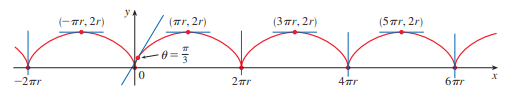
\includegraphics[width=0.8\textwidth]{graph28.png}
\end{figure}

(b) The tangent is horizontal when $\frac{dy}{d\theta}=r\sin\theta=0$ and $\frac{dx}{d\theta} \neq 0$. This occurs when $\theta = (2n+1)\pi$ for any integer $n$. The points are $(r(2n+1)\pi, 2r)$. The tangent is vertical when $\frac{dx}{d\theta}=r(1-\cos\theta)=0$, which is at $\theta=2n\pi$. However, at these points $\frac{dy}{d\theta}=0$ as well, so the curve has cusps.

\section*{Areas}
The area under a parametric curve is given by the formula:
\[
A = \int y \, dx = \int g(t)f'(t) \, dt
\]

\subsubsection*{EXAMPLE 3}
Find the area under one arch of the cycloid $x=r(\theta-\sin\theta)$, $y=r(1-\cos\theta)$.

\paragraph{Solution:}
One arch is traced as $\theta$ goes from $0$ to $2\pi$. We have $dx = r(1-\cos\theta)d\theta$.
\begin{align*}
    A &= \int_{0}^{2\pi} y \, dx = \int_{0}^{2\pi} r(1-\cos\theta) \cdot r(1-\cos\theta) \, d\theta \\
    &= r^2 \int_{0}^{2\pi} (1-\cos\theta)^2 \, d\theta = r^2 \int_{0}^{2\pi} (1 - 2\cos\theta + \cos^2\theta) \, d\theta \\
    &= r^2 \int_{0}^{2\pi} \left(1 - 2\cos\theta + \frac{1+\cos(2\theta)}{2}\right) \, d\theta \\
    &= r^2 \left[ \frac{3}{2}\theta - 2\sin\theta + \frac{1}{4}\sin(2\theta) \right]_{0}^{2\pi} = r^2 \left( \frac{3}{2} \cdot 2\pi \right) = 3\pi r^2
\end{align*}

\section*{Arc Length}
The length of a parametric curve is given by:
\[
L = \int \sqrt{\left(\frac{dx}{dt}\right)^2 + \left(\frac{dy}{dt}\right)^2} \, dt
\]

\subsubsection*{EXAMPLE 4}
Find the circumference of a circle $x=r\cos t, y=r\sin t$, for $0 \le t \le 2\pi$.

\paragraph{Solution:}
$\frac{dx}{dt} = -r\sin t$ and $\frac{dy}{dt} = r\cos t$.
\[
L = \int_{0}^{2\pi} \sqrt{(-r\sin t)^2 + (r\cos t)^2} \, dt = \int_{0}^{2\pi} \sqrt{r^2(\sin^2 t + \cos^2 t)} \, dt = \int_{0}^{2\pi} r \, dt = 2\pi r
\]

\subsubsection*{EXAMPLE 5}
Find the length of one arch of the cycloid $x = r(\theta-\sin\theta)$, $y = r(1-\cos\theta)$ for $0 \le \theta \le 2\pi$.

\paragraph{Solution:}
We have $\frac{dx}{d\theta} = r(1-\cos\theta)$ and $\frac{dy}{d\theta} = r\sin\theta$.
\begin{align*}
    L &= \int_{0}^{2\pi} \sqrt{r^2(1-\cos\theta)^2 + r^2\sin^2\theta} \, d\theta \\
    &= r \int_{0}^{2\pi} \sqrt{1 - 2\cos\theta + \cos^2\theta + \sin^2\theta} \, d\theta \\
    &= r \int_{0}^{2\pi} \sqrt{2 - 2\cos\theta} \, d\theta = r \int_{0}^{2\pi} \sqrt{4\sin^2(\theta/2)} \, d\theta \\
    &= \int_{0}^{2\pi} 2r\sin(\theta/2) \, d\theta = 2r \left[ -2\cos(\theta/2) \right]_{0}^{2\pi} \\
    &= -4r(\cos\pi - \cos 0) = -4r(-1 - 1) = 8r
\end{align*}

\section*{Speed and Length function}
The speed of a particle is $v(t) = s'(t) = \sqrt{(\frac{dx}{dt})^2 + (\frac{dy}{dt})^2}$.

\subsubsection*{EXAMPLE 6}
For a particle with position $x=2t+3, y=4t^2$ at $t \ge 0$, find the speed at the point (5,4).

\paragraph{Solution:}
The point (5,4) corresponds to $t=1$. The velocity components are $\frac{dx}{dt}=2$ and $\frac{dy}{dt}=8t$. At $t=1$, the speed is:
\[
v(1) = \sqrt{(2)^2 + (8(1))^2} = \sqrt{4+64} = \sqrt{68} = 2\sqrt{17}
\]

\section*{Surface Area}
The area of a surface generated by rotating a parametric curve about the x-axis is:
\[
S = \int 2\pi y \sqrt{\left(\frac{dx}{dt}\right)^2 + \left(\frac{dy}{dt}\right)^2} \, dt
\]

\subsubsection*{EXAMPLE 7}
Find the surface area of a sphere of radius $r$.

\paragraph{Solution:}
We use $x = r\cos t, y = r\sin t$ and rotate the upper semicircle ($0 \le t \le \pi$) about the x-axis.
\[
\sqrt{\left(\frac{dx}{dt}\right)^2 + \left(\frac{dy}{dt}\right)^2} = \sqrt{(-r\sin t)^2 + (r\cos t)^2} = r
\]
\begin{align*}
    S &= \int_{0}^{\pi} 2\pi (r\sin t) \cdot r \, dt = 2\pi r^2 \int_{0}^{\pi} \sin t \, dt \\
    &= 2\pi r^2 [-\cos t]_{0}^{\pi} = 2\pi r^2 (-\cos\pi - (-\cos 0)) = 2\pi r^2(1+1) = 4\pi r^2
\end{align*}

\end{document}